\chapter{Method of Approach}
\label{ch:method}

% This chapter should answer the ``how'' question - how did you complete your project, including the overall design of your study, details of the algorithms and tools you have used, etc.
%  Use technical diagrams, equations, algorithms, and paragraphs of text to
% describe the research that you have completed. Be sure to number all figures and tables and to explicitly refer to them in your text.

This project is about providing a new concept of recommend user potentially interested
music. Although it is only a munimal viable propotype, it would be good to make
it a web application hosted on a website. This chapter contains the tools utilized
for this application and the workflow for how do these tools work with each other.

\section{Tools Utilized}

The tools utilized for this application come from multiple areas. The general areas
can be catgorized with front-end area and back-end area. The following sub-sections
are the tools utilized.

\subsection{Flask}

Flask served as both front-end and back-end tool, it is a micro web application
framework, which means it does not require other third party libraries and services.
It is a stand along framework that you and add other parts onto it \cite{flask-documentation}.
Flask was implemented by Python, which is a great fit for this application because
this project processes a big amount of textual data. Python is famous for its
simple syntax and abundant of libraries, which means it is a good fit for big data
processing. Simple syntax means the code would be easy to read, and the processing
flow would be easily translated into actual code.

\subsubsection{Flask Front-end}

Flask uses HTML templates to render the front-end pages. Any values wants to be
changed dynamically when running the website can be passed into HTML files by using
variables. For example, in route functions, add the variable in return statement
as \ref{lst:html_var} shows. Then go to the redered HTML file, add \ref{lst:html}
in the corresponding place.

\begin{lstlisting}[language=Python, label={lst:html_var}, caption=Flask Route Template Variables]
return url_for(
  "html_file_name",
  outgoing_variable_name = incoming_variable_name,
  )
\end{lstlisting}

\begin{lstlisting}[language=HTML, label={lst:html}, caption=HTML Python Variables]
{{outgoing_variable_name}}
\end{lstlisting}

In general, HTML templates are the frame of the pages, Flask controls the dynamic
variables, and redering stratigies. In HTML files, \emph{form} were used to collect
user answers. As the code \ref{lst:form} shows.

\begin{lstlisting}[language=HTML, label={lst:form}, caption=HTML Forms]
<form method="POST">
  Title of text: <input type="text" name="title">
  <br>
  <textarea name = "text" rows="25" cols="80"></textarea>
  <br>
  <input type="submit" value="Submit">
</form>
\end{lstlisting}

\subsubsection{Flask Back-end}

In flask, modules can be imported by using Python importing statements.
All the setups can be put inside \emph{\_\_init\_\_.py} file for initialization. For
example, in \ref{lst:init}.

\begin{lstlisting}[language=Python, label={lst:init}, caption=Python Project Initialization]
from flask import Flask
from flask_sqlalchemy import SQLAlchemy
from flask_bcrypt import Bcrypt
from flask_login import LoginManager

# App Configurations
app = Flask(__name__)
# secret key to protect request and cookie
# use
# import secrets
# secrets.token_hex(16)
# to generate token.
app.config["SECRET_KEY"] = "__keys__"
# utilize db
app.config["SQLALCHEMY_DATABASE_URI"] = "sqlite:///site.db"
db = SQLAlchemy(app)
bcrypt = Bcrypt(app)
login_manager = LoginManager(app)

from music_main import routes
\end{lstlisting}

After imorted and seted up all the necessary libraries, they can be used as normal
Python programs. Other tools used in back-end will be explained in other sections
of this chapter.

\subsection{SQLAlchomy}

With such big amount of data, the best way of saving and retrieving data is by using
databases. Flask SQLAlchemy is a Flask extension that simplifies the implementation
of Structured Query Language (SQL) \cite{flask}. To create database by using Flask
SQLAlchemy, first initialize the library \ref{lst:utl}, then define the database
as models \ref{lst:db}. Use \ref{lst:create} to create database.

\begin{lstlisting}[language=Python, label={lst:utl}, caption=Flask SQLAlchemy Utilization]
app.config["SQLALCHEMY_DATABASE_URI"] = "sqlite:///site.db"
db = SQLAlchemy(app)
\end{lstlisting}

\begin{lstlisting}[language=Python, label={lst:db}, caption=Flask SQLAlchemy Model]
class User(db.Model, UserMixin):
    id = db.Column(
      db.Integer,
      primary_key=True,
    )
    username = db.Column(
      db.String(20),
      unique=True,
      nullable=False,
    )
    password = db.Column(
      db.String(60),
      nullable=False,
    )
    input = db.relationship("Input",
    backref="author",
    lazy=True,
    )

    def __repr__(self):
        return f"User('{self.username}')"
\end{lstlisting}

\begin{lstlisting}[language=Python, label={lst:create}, caption=Flask SQLAlchemy Create Database]
db.create_all()
\end{lstlisting}

\subsubsection{Relational Database}

This project used relational database to manage user data, lyrics data, and
processed data. The reason to choose relational database over non-relational
database is that the data used in this project is strictly structured. When comes
to trtriving resyults, it would be easier to use strictly defined tables. The data
used in this project can be devided into three tables. The user table stores usernames,
passwords, and its relation to other user data. The lyrics table stores the title of
the song, the singer of the song, the lyrics of the song, and the Summarization
of the lyrics. The input table stores the title of the user text, the user inputed
paragraphs, the Summarization of user input texts, and the top five results of
each text matching processing. The table design and their relations is as the graph
\ref{dbrela} shows.

\begin{figure}[htbp]
\centering
\includegraphics[width=2.5 in]{images/dbtable}
\caption{Database Design and Relation}
\label{dbrela}
\end{figure}

\subsection{Lyrics API}

All the lyrics this project used were coming from genius.com. Genius is a website
provides music music knowledge such as lyrics and story behind music \cite{genius}.
The developer website provides API to access their music knowledge.

\subsubsection{LyricsGenius}


LyricsGenius is a tool to retrive lyrics from genius.com on GitHub that was written
in Pyhton \cite{LyricsGenius}. This tool utilized Genius API to retrive song lyrics,
but user have to register Genius developer accout and then register for application
to get client access token. To get the lyrics, use \emph{search\_song} function
to get a Python object, then access the lyrics attribution. As the code \ref{lst:genius} shows.

\begin{lstlisting}[language=Python, label={lst:genius}, caption=LyricsGenius Sample Code]
import lyricsgenius

genius = lyricsgenius.Genius("my_client_access_token_here")
song = genius.search_song(song_title, song_artist)
song_lyrics = song.lyrics
\end{lstlisting}

Although this tool will return None when there is no song found accrding to the
search term, but the server would return vague results. Therefore, regular expression
was used to filter out these vague results.

\subsubsection{Playlists}

To get a list of song titles and song authors, a website called playlist-converter.net
\cite{playlist} was used to convert saved Spotify playlist into csv format files \ref{lst:csv}.
Then the file will be imported as Python list objects and will be further fed into
LyricsGenius tool. In this project, a total of 4 playlists with 593 pop songs was
added to the database. The name of the Spotify playlists are:
\emph{Happy Songs (80s, 90s, 2000s, 2010s \& 2020s \_  Best Happy Hits \& Oldies},
\emph{POP Music Playlist - Best POP Hits of All Time (Updated in 2020)},
\emph{Sad Songs},
and \emph{Top Pop}.

\begin{lstlisting}[label={lst:csv}, caption=Spotify Pliaylist]
"track","artist"
"Twist And Shout - Remastered","The Beatles"
"Uptown Funk (feat. Bruno Mars)","Mark Ronson"
"A-Punk","Vampire Weekend"
"Hooked on a Feeling","Blue Swede"
"Come","Jain"

...
\end{lstlisting}

\subsubsection{Language Detection}

For now, the only language model used was English, so, song language other than
English will also be filtered. Language detection tool, spacy-langdetect, based
on Spacy was used to detect whether the song lyrics is English \cite{langdetect}.
To use the tool, Spacy and Spacy English language model should be installed.
Then, use the Spacy and spacy-langdetect pipeline to create the object. As the
code sample \ref{lst:lang} shows.

\begin{lstlisting}[language=Python, label={lst:lang}, caption=Spacy Language Detection]
python -m spacy download en

import spacy
from spacy_langdetect import LanguageDetector

nlp = spacy.load('en')
nlp.add_pipe(
  LanguageDetector(),
  name='language_detector',
  last=True,
)
doc_check = nlp(text)
  if doc_check._.language["language"] == "en":
      return True
\end{lstlisting}

\subsection{Text Summarization}

To filter out the redundant texts and retain only the useful texts, a Python libray
called pytextrank was used to summarize each text entries. Pytextrank was implemented
based on Spacy pipline, and Mihalcea 2004 paper \cite{mihalcea2004textrank}, it
can rank the phrases and sentences \cite{pytextrank}. Based on the ranking, the
top phrases will be used to formulate the summarized sentences. To use pytextrank,
first install the dependencies, which are Spacy, NetworkX, and GraphViz. Then
download the Spacy English model. After add textrank into the Spacy pipeline,
import the text into the pipeline object. Finally, use \emph{summary} function
to get the Summarization of the text. As the sample code \ref{lst:textrank} shows.

\begin{lstlisting}[language=Python, label={lst:textrank}, caption=Pytextrank Sample Code]
python -m spacy download en_core_web_sm

import spacy
import pytextrank

nlp = spacy.load("en_core_web_sm")
tr = pytextrank.TextRank(logger=None)
nlp.add_pipe(tr.PipelineComponent, name="textrank", last=True)
doc = nlp(text)
whole_sent = ""
sum = doc._.textrank.summary(limit_phrases=15, limit_sentences=5)
for sent in sum:
  whole_sent = whole_sent + repr(sent).rstrip() + " "
\end{lstlisting}

\subsection{Text Matching}

There are many text maching algorithms, for example, Levenshtein, Jaccard index,
and cosine similarity. Although they all compare text entries, each algorithm only
has good proformance in certain areas. In situations like spelling check or keyword
search, Levenshtein would be a good fit. Levenshtein algorithm used Levenshtein
distance, it measures the minimum character edit steps from one string to another.
Similar algorithms are Hamming and Jaro-Winkler. They are called edit based similarities.
Edit based is simple and they are very effecient in short strings. However, they
do not consider the meaning of the strings. Algorithms such as Jaccard index and
cosine similarity are called token based similarities. The token here is a unit
of the string, for example, n-gram. They are effecient in long strings, and they
take the meaning of the text into account. However, they are not very effecient
in short strings. These algorithms are good fit for areas such as text mining and
bioinfomatics.

This project used a hybrid algorithm called Monge-Elkan. It combines both edit
based similarities and token based similarities. It combined the advantages of edit
based similarities and token based similarities. However, they can be slower than
other similarity check algorithms. The tool this project used is called py\_stringmatching.
It has a module to compute the Monge-Elkan similarity of two strings \cite{matching}.

To use py\_stringmatching, first import the library. Then initialize the \emph{MongeElkan}
function. Finally, use the \emph{get\_raw\_score} function to compare two string
entries. As the sample code \ref{lst:monge} shows.

\begin{lstlisting}[language=Python, label={lst:monge}, caption=Monge-Elkan Similarity]
import py_stringmatching as sm

me = sm.MongeElkan()
return me.get_raw_score(user_sum, lyrics_sum)
\end{lstlisting}

\section{Implementation and Workflow}

This section explained how does the project organized and how were the tools used
to construct the application. The workflow of the project is also explained in
this section.

\subsection{Project Implementation}

This subsection explained the prerequisites, library management, and file structure
of the project.

\subsubsection{System and Python Versions}

This project was implemented and deployed on Linux system. Specifically Ubuntu
18.04.4 LTS \ref{lst:linux}.

\begin{lstlisting}[language=bash, label={lst:linux}, caption=System Version]
cat /proc/version
Linux version 4.15.0-76-generic (buildd@lcy01-amd64-029)
(gcc version 7.4.0 (Ubuntu 7.4.0-1ubuntu1~18.04.1))
#86-Ubuntu SMP Fri Jan 17 17:24:28 UTC 2020
\end{lstlisting}

The Python version used was Python 3.7.6 \ref{lst:pyver}. To implement the project
with the desired Python version, Pyenv was used to avoid version conflict between
installed version of Python with system versions of Python. Pyenv is a simple but
powerful Python version management tool \cite{pyenv}. This tool can be used to
download desired versions of Python easily. The scope of the Python can be set to
global, which means the desired version of Python can be used system-wise, or local,
which means the desired version of Python can only be used in a specific project.

\begin{lstlisting}[language=bash, label={lst:pyver}, caption=Python Version]
pyenv versions
  system
* 3.7.6 (set by /home/sheldon/.pyenv/version)
\end{lstlisting}

\subsubsection{Library Management}

Many tools and plugins was used in this project. To avoid the dependency confliction,
Pipenv was used to manage the packaging. Pipenv is a dependency management tool \cite{pipenv}.
With pipenv, all the specification can be recorded in \emph{Pipfile} \ref{lst:pipfile}.
For example, Python version, dependencies, customized scripts.

\begin{lstlisting}[label={lst:pipfile}, caption=Pipenv Pipfile]
[[source]]
name = "pypi"
url = "https://pypi.org/simple"
verify_ssl = true

[dev-packages]

[packages]
lyricsgenius = "==1.8.2"
spacy = "==2.2.4"
networkx = "==2.4"
graphviz = "==0.13.2"
pytextrank = "==2.0.1"
numpy = "==1.18.2"
pip = "*"
six = "==1.14.0"
py-stringmatching = "==0.4.1"
spacy-langdetect = "==0.1.2"
attrs = "==19.3.0"
bcrypt = "==3.1.7"
beautifulsoup4 = "==4.6.0"
blis = "==0.4.1"
catalogue = "==1.0.0"
certifi = "==2019.11.28"
cffi = "==1.14.0"
chardet = "==3.0.4"
click = "==7.1.1"
coverage = "==5.0.4"
cymem = "==2.0.3"
decorator = "==4.4.2"
idna = "==2.9"
importlib-metadata = "==1.5.0"
itsdangerous = "==1.1.0"
langdetect = "==1.0.7"
more-itertools = "==8.2.0"
murmurhash = "==1.0.2"
plac = "==1.1.3"
pluggy = "==0.13.1"
preshed = "==3.0.2"
py = "==1.8.1"
pycparser = "==2.20"
pyparsing = "==2.4.6"
pytest = "==5.4.1"
requests = "==2.23.0"
srsly = "==1.0.2"
thinc = "==7.4.0"
tqdm = "==4.43.0"
urllib3 = "==1.25.8"
wasabi = "==0.6.0"
wcwidth = "==0.1.8"
zipp = "==3.1.0"
Flask = "==1.1.1"
Flask-WTF = "==0.14.3"
Flask-SQLAlchemy = "==2.4.1"
Flask-Bcrypt = "==0.7.1"
Flask-Login = "==0.5.0"
Jinja2 = "==3.0.0a1"
MarkupSafe = "==1.1.1"
SQLAlchemy = "==1.3.15"
Werkzeug = "==1.0.0"
WTForms = "==2.2.1"
gunicorn = "*"

[requires]
python_version = "3.7"

[scripts]
music = "./scripts/music.sh"
setup = "./scripts/setup.sh"

[pipenv]
allow_prereleases = true
\end{lstlisting}

With Pipenv, Python vertual environment can be set up and denpencies with users'
required version can be install easily and recorded into Pipfile by using one line
of bash command. If there are any confliction between denpendencies, Pipenv can
also help to diagnose the confliction and provides resolving advises. A complete
list of requirements in the requirement file is as follows \ref{lst:req}:

\begin{lstlisting}[label={lst:req}, caption=requirements.txt]
-i https://pypi.org/simple
attrs==19.3.0
bcrypt==3.1.7
beautifulsoup4==4.6.0
blis==0.4.1
catalogue==1.0.0
certifi==2019.11.28
cffi==1.14.0
chardet==3.0.4
click==7.1.1
coverage==5.0.4
cymem==2.0.3
decorator==4.4.2
flask-bcrypt==0.7.1
flask-login==0.5.0
flask-sqlalchemy==2.4.1
flask-wtf==0.14.3
flask==1.1.1
graphviz==0.13.2
idna==2.9
importlib-metadata==1.5.0 ; python_version < '3.8'
itsdangerous==1.1.0
jinja2==3.0.0a1
langdetect==1.0.7
lyricsgenius==1.8.2
markupsafe==1.1.1
more-itertools==8.2.0
murmurhash==1.0.2
networkx==2.4
numpy==1.18.2
packaging==20.3
plac==1.1.3
pluggy==0.13.1
preshed==3.0.2
py-stringmatching==0.4.1
py==1.8.1
pycparser==2.20
pyparsing==2.4.6
pytest==5.4.1
pytextrank==2.0.1
requests==2.23.0
six==1.14.0
spacy-langdetect==0.1.2
spacy==2.2.4
sqlalchemy==1.3.15
srsly==1.0.2
thinc==7.4.0
tqdm==4.43.0
urllib3==1.25.8
wasabi==0.6.0
wcwidth==0.1.8
werkzeug==1.0.0
wtforms==2.2.1
zipp==3.1.0
\end{lstlisting}

\subsubsection{File Structure}

The project repository contains the application directory. This directory has the
HTML templates, application Python files, and the database file. The playlist
directory contains all the Spotify playlists. The scripts directory contains the
script to set up the environment and download the dependencies automaticlly then
start the service. Test directory contains all the testing program for the application.
Texts directory contains all the input files wrote by the users. In the project
root directory, there are app main function file, Pipfile, Piplock file, and requirements
record text file.

The file structure of this project is as follows \ref{tree}:

\begin{figure}[htbp]
\centering
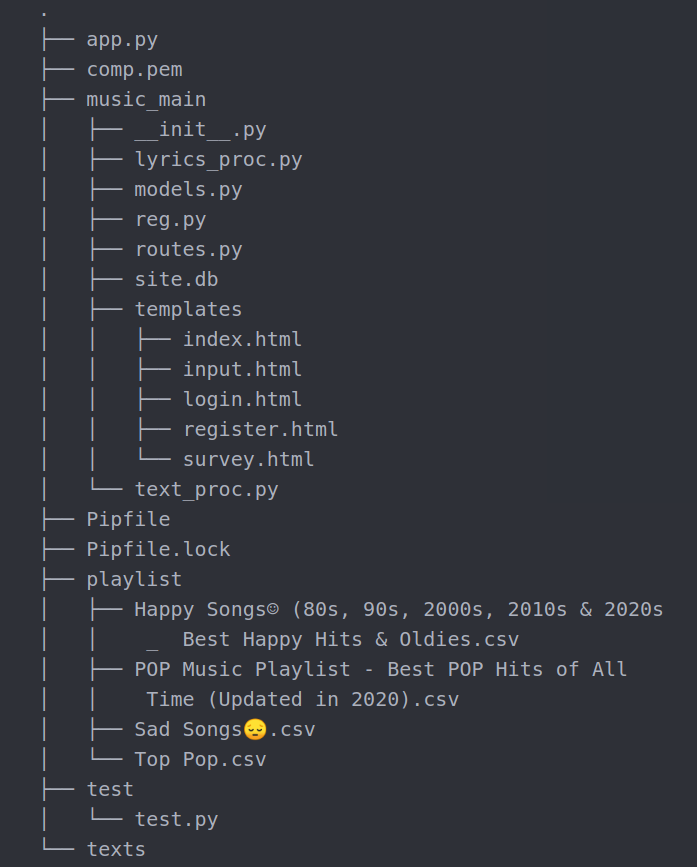
\includegraphics[width=6 in]{images/file-tree}
\caption{File Structure Tree}
\label{tree}
\end{figure}

\subsection{Workflow}

This section explained the deployment steps of this project, workflow of the process,
and the user access flow.

\subsubsection{Deployment}

After finised the implementation, the project Pipfile was locked, which means all
the dependency versions was locked. To automate the setup process on new environment,
a script was added to the project. Under script section of Pipfile, add the command
keyword and the path of the script, for example, \emph{setup = "./scripts/setup.sh"}.
The command to setup a new environment would be \emph{pipenv run setup}. In the
setup script, there were command to download the two English language models, from
Spacy, the command to create the databases, and the command to run the Lyrics
model to update the Lyrics table with lyrics from Genius, and summarization of each
lyrics. The Bash script is as follows \ref{lst:setup}:

\begin{lstlisting}[language=bash, label={lst:setup}, caption=setup.sh]
#!/bin/bash

# Download language model
pipenv run python -m spacy download en_core_web_sm
pipenv run python -m spacy download en
# create database
pipenv run python -c "from music_main import db; \
from music_main.models import User, Input, Lyrics; \
db.create_all()"
# Create data for Lyrics table
pipenv run python -c \
"from music_main.lyrics_proc import *; lyrics_main()"
\end{lstlisting}

After the above preperations, ssh into the server and clone the repository from
GitHub. Install the Pyenv and then the version of Python used to implement the
Project. Install the Pipenv, and use \emph{pipenv install} to create Python vertual
environment and install all the denpendencies according to the Pipfile. Nginx and
Gunicorn was used as web servers during deplyment on Amazon AWS server. Supervisor
was used to moniter the application process on the Amazon AWS Linux server.

\subsubsection{Workflow}

When everything is ready and the application is up and running on the server, the
URLof the website can be shared to people who are interested in participating the
experiment.

When lyrics model was ran during the deployment process, the playlist was first
combined into one list. Then the list was loop through and was used to get the
lyrics from Genius by using lyricsgenius library. After making sure the result
was real lyrics and the language was English by using regular expression and
spacy-langdetect, the lyrics was summarised by calling summarization function
powered by Pytextrank from text model. Finally, the corresponding information was
added and committed to the database table.

After user filled in their response, the text was saved as text files, and the
summarization function was called from the text model. Then the text matching
function powered by py-stringmatching was also called from the text model. The
top 5 results was kept, and all the corresponding information was saved into the
database table.

The complete system design is as graph \ref{sys} shows.

\begin{figure}[htbp]
\centering
\includegraphics[width=6 in]{images/sys}
\caption{System Design}
\label{sys}
\end{figure}

\subsubsection{Access Flow}

When users access the website to use the application and to participate the experiment,
the landing page will contain the brief project Introduction, data usage, how to
quit the experiment anytime, compensation lottary participation, experimentor contact
information, log in link, log out link, and register link. As the graph \ref{landing} shows.
After user registered and logged in, user will be landed in the user input page \ref{input}.
Here user will read the instruction and fill out the blanks. In the result page,
a list of no more than 5 songs will be shown to the user, followed by the link to
the survey and compensation participation sign up link \ref{result}. The sitemap
of this application is as graph \ref{sitemap} shows. The Walk-Through section under
Experiments also talked about the access flows.

\begin{figure}[htbp]
\centering
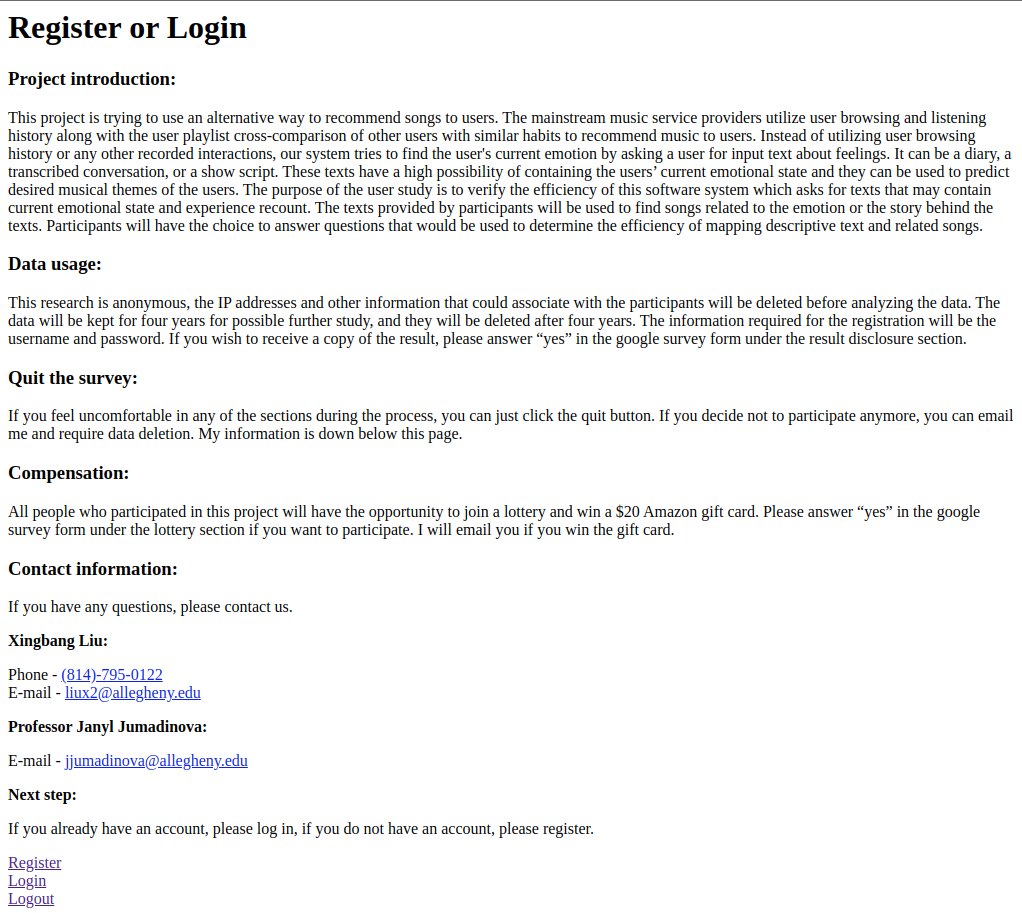
\includegraphics[width=6 in]{images/landing}
\caption{Landing Page}
\label{landing}
\end{figure}

\begin{figure}[htbp]
\centering
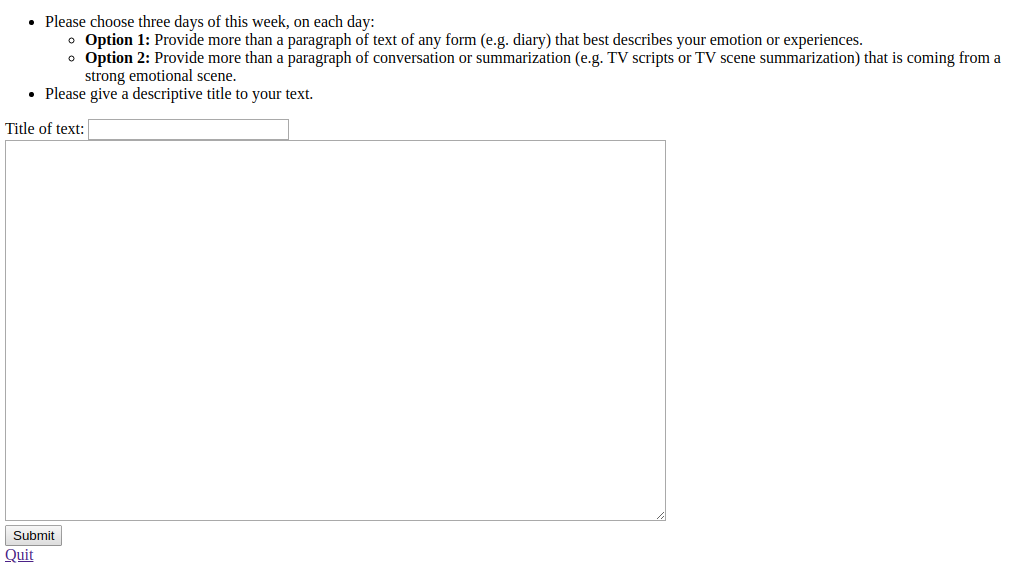
\includegraphics[width=6 in]{images/input}
\caption{Input Page}
\label{input}
\end{figure}

\begin{figure}[htbp]
\centering
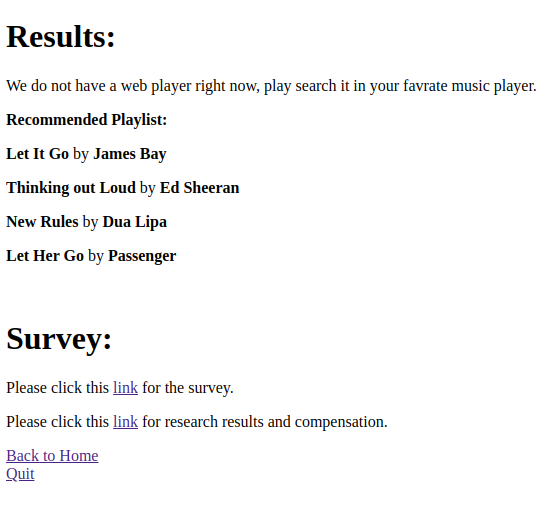
\includegraphics[width=6 in]{images/result}
\caption{Result Page}
\label{result}
\end{figure}

\begin{figure}[htbp]
\centering
\includegraphics[width=6 in]{images/sitemap}
\caption{Sitemap}
\label{sitemap}
\end{figure}
